\section{View}
The UI will be looking like: \\
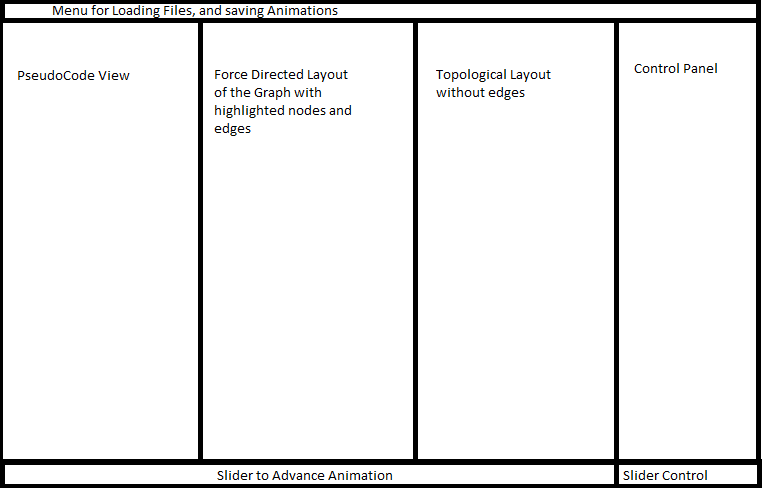
\includegraphics[width=\textwidth]{parts/UIFinished}
\begin{list}{-}{}
\item The left Section will be showing the pseudocode of the current active algorithm.
\item The Middle Sections will show one force directed  graph on the left that will higlight Nodes the right will be ordered Topological.

\item Nodes will be a default size.
\item Nodes in both graphs will be coloured dynamically.
\begin{list}{-}{}
\item Currently used node will be coloured green. (left Graph)
\item Sources will be colured cyan.
\item Sinks will be colured light gray.
\end{list}
\item Edges will be coloured as following.
\begin{list}{-}{}
\item Active edge will be coloured blue.
\item Reversed edges will be coloured green.
\end{list}
\item The right section will be a Control Panel.
\begin{list}{-}{}
\item for more information see Section Controller

\end{list}
\end{list}




